%MRC5December2012 -- Added a bit about  the corporate partner context
%Context
\chapter{Context}
\label{sec-context} %Label for cross-referencing

%%%%%%%%%%%%
\begin{remark} \color{blue}
Suggested length: half a page to a page each for the Need Statement and Problem Statement (plus figures, if any). Another page or two for the design team.
\vspace{0.1in}

\noindent The Context provides background and motivation for your project. It is an enlarged version of the brief context in your Executive Summary.  
\begin{itemize} \tightlist
\item Who came to you with a proposed project area? Who is the corporate partner and what is their context?
\item What background or context set the stage for your Needfinding and Benchmarking, activities?
\end{itemize}
\normalcolor \end{remark}
%%%%%%%%%%%%

\section{Need Statement}
\label{sec:need}

%%%%%%%%%%%%
\begin{remark} \color{blue}
This section is the high-level result of your user need-finding. It provides the background for the ``Point of View'' or hypothesis that guides your ongoing work. 
\begin{itemize} \tightlist
\item Who wants or needs your product? Why do they want it? Or, what need does the product area address? 
\item What evidence do you have to substantiate the need? Use citations or other evidence you've gathered.
\end{itemize}

\noindent The remaining text is taken from \cite{Autodesk2008Fall}.
\normalcolor \end{remark}
%%%%%%%%%%%%

The design world has changed dramatically in the last decade. The widespread advancement and usage of digital prototyping tools has made it simpler and faster to realize new ideas. At the same time, globalization is requiring designers from remote locations to combine their ideas and make design decisions. 

With the advancement of computational power and communication speed, digital prototyping tools have made it possible to transmit complex drawings around the world. Most digital tools that promote remote collaboration target the idea-to-conception stage of development. The early ideation stages of engineering design, however, are still more effective when discussed locally. The problems of effective communication and effective decision-making in this setting are still largely unsolved. Internet tools setup the virtual meeting space, yet communication is still not as effective as meeting in the same room. Often meeting participants cannot truly work together as they do face-to-face.

Wouldn't it be perfect to have a new tool that focused on the interaction aspects of remote collaboration? A tool that made communication effortless, as if the participants were in the same room. Such a tool could increase the ideation potential of remote meetings and make remote brainstorming a reality. 

\section{Problem Statement}
\label{sec:problem}

%%%%%%%%%%%%%%%
\begin{remark} \color{blue}
Here you get more specific about the particular problem that your design vision is addressing.
The remaining text is again taken from \cite{Autodesk2008Fall},
\normalcolor \end{remark}
%%%%%%%%%%%%%%%

In order to facilitate remote collaboration in the early design stage, we first break down the problem into the following three areas.

\begin{itemize} \tightlist
\item Social Dynamics
\item Communication tools
\item Idea storage and decision making
\end{itemize}

Early ideation is a very social process and requires effective interperson communication. Current teleconferencing tools lack in recreating the level of social dynamics present in face-to-face communication.

Communication tools are a means with which we transmit ideas to each other. This could be either through speaking, body language, or drawing. The early ideation stage requires a rapid exchange of ideas between all participants in a meeting. How can we utilize communication tools effectively to make such a dialog easier?

Finally, the brainstorming stage presents a plethora of ideas that need to be archived and categorized for effective decision making. How can we make it easier for meeting participants to save their ideas and retrieve them later? How can information be viewed to facilitate decision making?

\section{Corporate partner: Autodesk}

%%%%%%%%%%%%%%%
The corporate partner for this project is Autodesk Corp.
Since 1982, Autodesk has delivered 2D and 3D visualization tools for clients in manufacturing and design. Well known products include the drafting program AutoCAD
, digital prototyping software Inventor, and 3D modeler Maya. The company focuses on enhancing the design process by allowing the customer to experience their design through software. Increasingly, Autodesk is interested in 
tools for portable computing (e.g. tablets) and for integrated solutions that allow design, video collaboration, data management, etc.

\begin{remark} \color{blue}
Add a bit more about the corporate partner and their context, perhaps using the information you started to obtain in the Business 
Canvas exercise, as introduced in class. A couple of good examples can be found in the 2012 Spring documents from Electric Mobility Norway \cite{EMN2012Spring} and Symbiose\'{e} \cite{Symbiosee2012Spring}.
%See also the new suggested ``Venture Requirements'' (Section \ref{sec:venturereqs}).
\normalcolor \end{remark}

\subsection{Corporate Liaisons}
Say who the liaisions are and give their contact information.

%%%%%%%%%%%%%%%%%%%%%%%%%%%%%%%%%%%%%%%%%%%%%%%%%%

\section{The Design Team}
\label{sec:team}

%%%%%%%%%%%%%%%%%%%
\begin{remark} \color{blue}
See other recent reports for other ways of introducing the team. To the extent that the characteristics of the team influence the project direction, this is of interest to the reader.
\end{remark} \normalcolor
%%%%%%%%%%%%%%%%%%%

Team \pmt, was assembled from individuals with a diversity of thinking preferences, interests and backgrounds. There is some evidence that such diversity enhances team creativity \cite{Wilde97} \cite{Wilde07}, even if it creates additional challenges for team management.

% Example table. It gets a caption and reference label.
% The tabular formatting is a bit painful...  An alternative is to use Word
% and insert the PDF printout as for a figure. There are also Word-to-Latex converters.
%
%Nov2013 -- I decided to comment this out because corporate partners don't care about this. -MRC
%
%\begin{table}
%  \begin{tabular}{| p{14mm} | p{20mm} | p{20mm} | p{22mm} | p{20mm} | p{12mm} |} 
%  \hline
%Score & Extroverted-Introverted (E-I) & Intuition-Sensing (N-S) & Feeling-Thinking (F-T) & Perception-Judging (P-J) & Overall \\
%People & & & & &\\
%\hline
%Larry & +6 & +6 & -6 & +12 & ENTP \\
%Mark & -18 & +30 & -30 & +18 & INTP \\
%George & +6 & +18 & -18 & +6 & ENTP \\
%\hline
%\end{tabular}
%\caption{Team preferences scores using the method of Wilde \cite{Wilde07}. (These data are not real.)}
%	\label{wildeprefs}  %Tag for referring to table
%\end{table}

\begin{framed}
\noindent 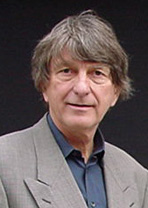
\includegraphics[width=40mm]{Figures/Ch2/LarryLeifer.jpg}
\parbox[b]{0.6\textwidth}{Larry Leifer\\
Status: Professor, Mechanical Engineering\\
Contact: leifer@cdr.stanford.edu\\
Skills: deisgn, mechatronics, welding, prototyping\\
Computing: Solid Works, Matlab, basic C programming, Forth\\
}
%Note, the blank lines matter - they cause the start of a paragraph in the box.

Born in Santa Barbara I remain a surfer at heart.
My research is focused on instrumenting, understanding, supporting, and improving design practice through the development of design theory. BS in in Engineering Science, MS in Product Design, PhD in Biomedical Engineering, all from Stanford.
Founder of the  Center for Design Research and one of the founding faculty members of the Hasso Plattner Design Institute
at Stanford (aka the d.school).

Favorite activities include surfing, hunting and wayfaring, and frequent trips to Lucerne, Switzerland.
\end{framed}

\begin{framed}
\noindent 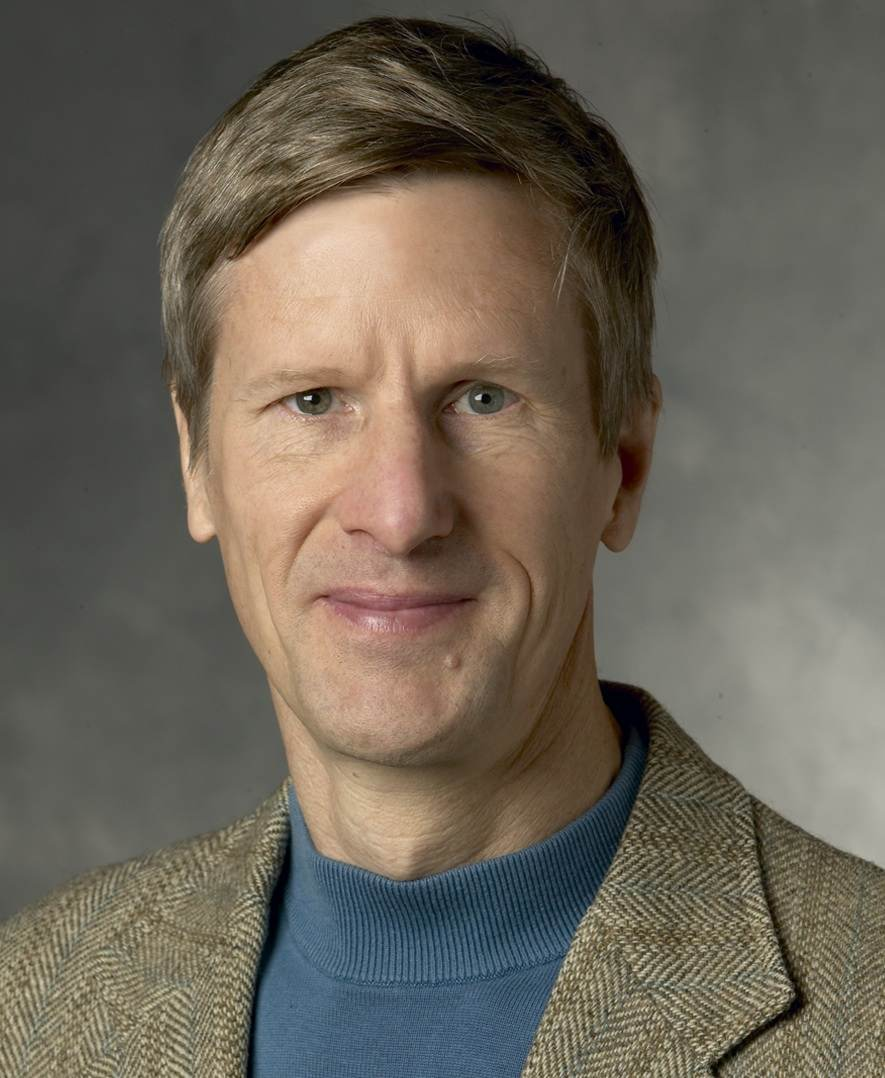
\includegraphics[width=40mm]{Figures/Ch2/MarkCutkosky}
\parbox[b]{0.6\textwidth}{Mark Cutkosky\\
Status: M.E. Graduate Student\\
Contact: cutkosky@stanford.edu\\
Skills: woodworking, masonry, soldering, Lasercamm\\
Computing: Matlab, C, Python, Perl, Inkscape, basic Unix\\
}

Born and raised in Pittsburgh PA, I worked at ALCOA as a machine designer before getting my Ph.D. from Carnegie Mellon University in Robotics. My research applies analyses, simulations, and experiments to the design and control of bio-inspired robots, robotic hands, tactile sensors, and devices for human/computer interaction. In manufacturing, my work focuses on multi-material rapid prototyping methods. \\
My lab: \url{http://bdml.stanford.edu}

\end{framed}

\begin{framed}
\noindent 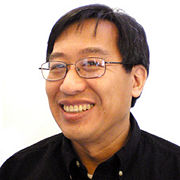
\includegraphics[width=40mm]{Figures/Ch2/GeorgeToye}
\parbox[b]{0.6\textwidth}{George Toye\\
Status: Consulting Professor, Mechanical Engineering\\
Contact: deputy@me310.stanford.edu\\
Skills: machining, welding, foreign languages\\
Computing: Solid Works, Assembler, Eagle, various computer languages\\
}

Originally from Taiwan, I grew up in Montreal and San Francisco.  BSME from U.C. Berkeley and Ph.D. from Stanford in M.E. I have also worked in various Bay Area consulting and high technology startup firms. My expertise includes mechatronics (I have sometimes taught ME218) and Unix/Linux server management.  My own company is  \url{http://www.withinc.com/}.

\end{framed}

\subsection{Coach}

Say who your team's coaches are and give some basic information and contact information.

%%%%%%%%%%%%%%%%%%MORE LATEX EXAMPLES%%%%%%%%%%%%%%
% Let's test some in-situ glossary items. The idea is to insert these kinds of definitions anywhere,
% as they occur to you while incrementally working on the documentation.
%See main file for notes about how to convert the ".glo" file to a glossary section.

\glossary {paper weight}{ the combined weight of all paper products (paper, cardboard, crepe paper, paper tape) in the vehicle.}
\glossary {non-paper weight}{ the combined weight of all non paper items (e.g. metal pins, teflon tape, screws). Non-paper weight is severely restricted in ME310 Paper Bike exercises.}
\glossary {papier m\^{a}ch\`{e} }{a composition of shredded paper glued together with library paste}
\glossary {particle board} {a product made of compressed wood chips and resin, often sold in 4 ft x 8 ft sheets. Particle board is not considered a paper product.}
\glossary {sound deadener board} {a product made of compressed cardboard fibers and resin, often sold in 4 ft x 8 ft sheets. Sound deadener board is not considered a paper product.}

\begin{remark} \color{blue}
\section*{Experiments with tables in Latex}

Here is a centered tabular form that is 3/5 of the current text width and has a horizontal line but no
vertical lines:

 \begin{center}  % put inside center environment
  \begin{tabular*}{0.6 \textwidth}%
     {@{\extracolsep{\fill}}cccr}
  \multicolumn{3}{c}{a label spanning 3 merged cells} & label 4  \\
  \hline  % put a line under headers
  item 1a  & item 2a  & item 3a  & item 4a  \\
  item 1b  & item 2c  & item 3c  & item 4c  \\
  \end{tabular*}
  \end{center}

\noindent For anything more complicated than the examples in this section, it may be easiest to do the table in MS Word or OpenOffice, create a pdf and include the pdf in a table environment. Because pdf files have scalable fonts, the print resolution will be good.
For example, Table \ref{tab:physical-requirements} is taken from an Audi fall document \cite{Audi2009Fall} done in MS Word and pasted as PDF into Latex. Notice that the fonts are scalable if you zoom in.

\begin{table}[h]
	\centering
		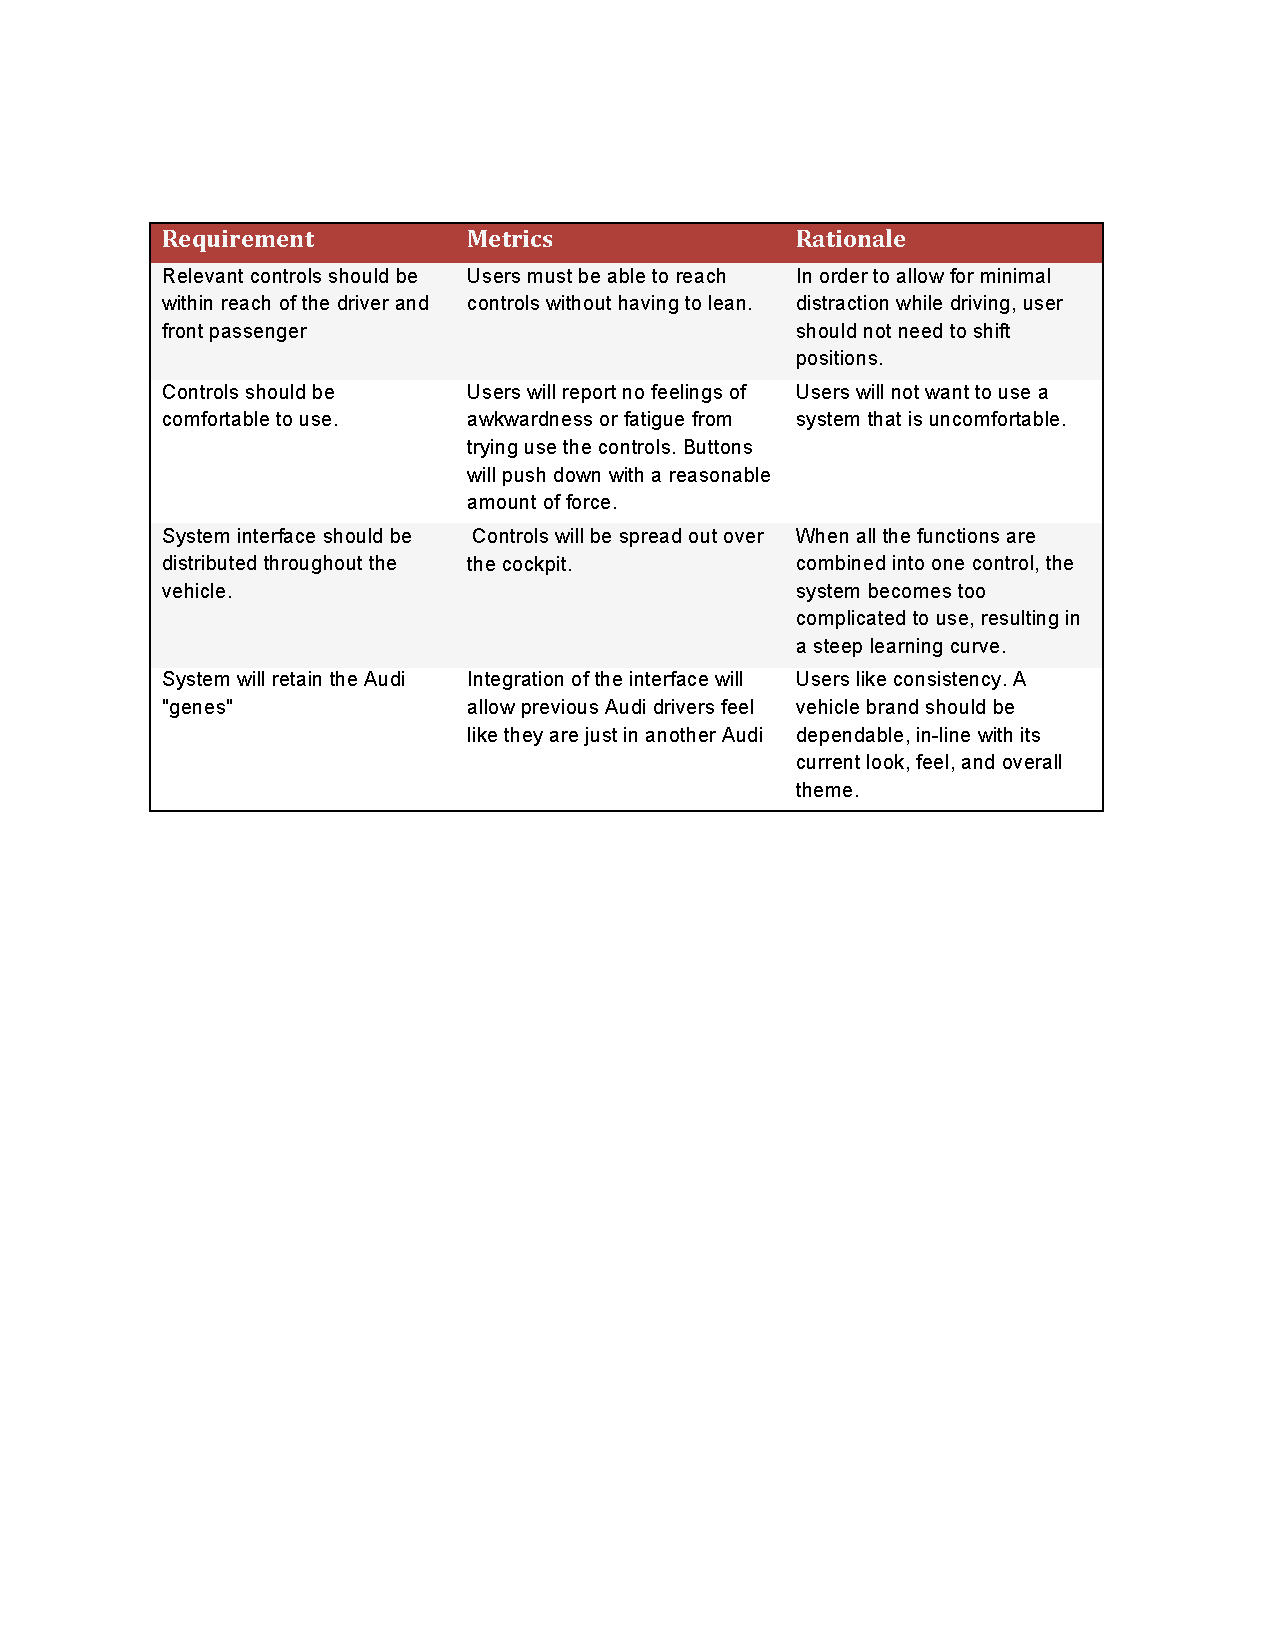
\includegraphics[width=\textwidth]{Figures/Ch3/Audi08PhysReqs.pdf}
	\caption[A PDF table]{Physical Requirements from \cite{Audi2009Fall}, used here just to illustrate how PDF can be pasted in as a table
	}
	\label{tab:physical-requirements}
\end{table}

\end{remark}\normalcolor
